% !Mode:: "TeX:UTF-8"
\documentclass[master,openright,twoside,color]{buaathesis}
\usepackage{booktabs}
\usepackage{graphicx}
\begin{document}

% 用户信息
% !Mode:: "TeX:UTF-8"

% 学院中英文名,中文不需要“学院”二字
% 院系英文名可从以下导航页面进入各个学院的主页查看
% http://www.buaa.edu.cn/xyykc/index.htm
\school
{XXX}{School of XXX}

% 专业中英文名
\major
{XXXX}{XXXX Engineering}

% 论文中英文标题
\thesistitle
{基于Texlive的北航毕设论文模板设计长标题长标题长标题长标题}
{这里是长长的长长的长长的长长的长长的长长的长长的长长的长长的副标题}
{How to design the BUAA-thesis with \LaTeX{} very very very very very very long}
{English sub title, It is very very very very very very very very very very long}

% 作者中英文名
\thesisauthor
{姓名}{Name}

% 导师中英文名
\teacher
{导师中文名}{Name of tutor}
% 副导师中英文名
% 注:慎用‘副导师’,见北航研究生毕业论文规范
%\subteacher{副导师}{subteacher}

% 中图分类号,可在 http://www.ztflh.com/ 查询
\category{TP312}

% 本科生为毕设开始时间;研究生为学习开始时间
\thesisbegin{2011}{09}{01}

% 本科生为毕设结束时间;研究生为学习结束时间
\thesisend{2012}{07}{01}

% 毕设答辩时间
\defense{2012}{06}{01}

% 中文摘要关键字
\ckeyword{北航开源俱乐部,\LaTeX{},论文}

% 英文摘要关键字
\ekeyword{BHOSC, \LaTeX{}, Thesis}

% !Mode:: "TeX:UTF-8"

% 研究方向
\direction{大数据和云计算}

% 导师职称中英文
\teacherdegree{教授}{Prof.}
% 副导师职称中英文
% 注:慎用‘副导师’,见北航研究生毕业论文规范
%\subteacherdegree{讲师}{Teacher}

% 保密等级,注:非保密论文时不需要此项
%保密论文请更改‘buaathesis.cls’里相应代码
%\mibao{机密}

%申请学位级别
\applydegree{全日制工程硕士}

% 论文编号,由10006+学号组成
\thesisID{10006SY0000000}

% 论文提交时间
\commit{2012}{03}{03}

% 学位授予日期
\award{2012}{04}{04}


% 中英封面、提名页、授权书
\maketitle
% 前言页眉页脚样式
\pagestyle{frontmatter}
% 摘要
\begin{cabstract}
我做了中文摘要
\end{cabstract}

\begin{eabstract}
Abstract  in English.
\end{eabstract}
% 目录、插图目录、表格目录
\tableofcontents
\listoffigures
\listoftables
% 符号表
%% !Mode:: "TeX:UTF-8"
\begin{denotation}

\item[HPC] 高性能计算 (High Performance Computing)
\item[cluster] 集群
\item[Itanium] 安腾
\item[SMP] 对称多处理
\item[API] 应用程序编程接口
\item[PI] 聚酰亚胺
\item[MPI] 聚酰亚胺模型化合物,N-苯基邻苯酰亚胺
\item[PBI] 聚苯并咪唑
\item[MPBI] 聚苯并咪唑模型化合物,N-苯基苯并咪唑
\item[PY] 聚吡咙
\item[PMDA-BDA] 均苯四酸二酐与联苯四胺合成的聚吡咙薄膜
\item[$\Delta G$] 活化自由能~(Activation Free Energy)
\item[$\chi$] 传输系数~(Transmission Coefficient)
\item[$E$] 能量
\item[$m$] 质量
\item[$c$] 光速
\item[$P$] 概率
\item[$T$] 时间
\item[$v$] 速度
\end{denotation}


% 正文页码样式
\mainmatter
% 正文页眉页脚样式
\pagestyle{mainmatter}

% 正文
% !Mode:: "TeX:UTF-8"
\chapter{简介}
\section{论文工作计划}
\subsection{论文研究目标}
近年来,随着 Internet 的兴起,互联网上的数据急剧膨胀。根据国际数据信息公司\footnote{https://www.idc.com/}(International Data Corporation, IDC)的统计和预测,2017 年全球网络数据量已经达到1.8ZB,到2025 年,全球数据总量预计还将增长50 倍。大量无标注数据的出现,也让研究人员开始考虑,如何利用算法从这些大规模无标注的文本数据中自动挖掘规律,得到有用的信息。自从2006年,加拿大多伦多大学教授 Geoffrey Hinton 提出的深度学习(Deep Learning, DL)概念以来\cite{hinton2006reducing},为解决如何利用爆炸的数据量,以提取有效知识带来了新的思路。在这之后的发展中,基于神经网络的表示学习技术(Representation Learning)开始在各个领域崭露头角。尤其在图像(Image Classification)和语音(Automatic Speech Recognition)领域的多个任务上,基于表示学习的方法在性能上均超过了传统基于特征提取(Feature Extraction)的方法。

近年来,深度学习技术(Deep Learning)逐渐在自然语言处理中(Natural Language Processing, NLP)得到应用。 例如,蒙特利尔大学教授 Yousha Bengio 提出用神经网络(Neural Network, NN) 来训练语言模型(Language Model)并进行了相关探索\cite{DBLP:conf/nips/BengioDV00}。 后续的工作中,基于循环神经网络(Recurrent Neural Network, RNN)的语言模型建模方法由其学生 Tomas Mikolov 进行了极大拓展和完善\cite{DBLP:conf/interspeech/MikolovKBCK10}。 网络通过学习能够将当前词的历史信息存储起来,以词的整个上下文(Context)作为依据,来预测下一个词出现的概率,克服了 N-gram 语言模型无法利用语句中长距离上下文依赖(Long Term Dependency)的缺点。 另外,在模型训练的过程中,由于词的历史信息被映射到低维连续空间,语义相似的词被聚类,在语料中出现次数较少的词仍然能够得到很好的训练,不再需要额外的数据平滑技术(Smoothing Technology)。
迄今为止,采用RNN 训练的语言模型在模型困惑度(Perplexity, PPL)和识别系统的识别率上都取得了最好的效果。 RNN 建模方法虽然表现出极大的优越性,却以牺牲计算复杂度为代价。 若训练大规模的文本语料,则需要花费很长的时间,制约了RNN 语言模型训练效率。 为克服这一不足,文献 \cite{DBLP:conf/icassp/MikolovKBCK11} 提出了多种优化策略来降低网络的计算复杂度,如缩短模型训练周期、减少训练数据集的规模、降低训练词表(Vocabulary)的大小、减少隐含层的节点数等,这些方法都在一定程度上降低了网络的运算量,提高了模型的训练效率,但同时也牺牲了较多的模型性能。 另外,在网络结构层面上,文献\cite{DBLP:journals/coling/BrownPdLM92} 研究了一种基于分类的循环神经网络(Class-based RNN) 结构,网络的输出层被分解为两部分,增加的一部分称为分类层,从结构上降低了整个网络的计算复杂度,使得模型训练效率有了一定的提升且模型性能没有大的变化。 然而,在大词汇量连续语音识别系统中,采用此结构训练大规模语料语言模型仍需要花费大量时间。 因此,模型训练效率有待进一步优化。

\subsection{论文主要研究内容}
语言模型的大词表问题是目前理论应用到实际过程中必须要克服的问题,我们当然可以通过配置高性能服务器来暂时延缓该问题的后果。但是一旦应用到大数据集上,即使是目前最好的中央处理器(CPU)或者图形处理器通用计算(GPU),仍然需要一个多月时间才能训练完善。因此,在保证原有模型的准确率和精度的前提下,如何提高模型的训练速度是我们主要讨论和研究的内容。为此我们讨论了两个不同的内容:上下文信息建模效率和精度对比和大词表问题的优化和研究。

针对上下文信息建模手段,目前主要采用的方案有以下几种:

一种是采用子词(Subword)或者字符级别的词(Character-level)来直接缩小词表大小;一种是通过采样技术(Sampling-based Approximation)来减少必要的训练时间;一种是通过基于分类的多元分类(class-based hierarchical softmax, cHSM)来加速模型和采用基于树模型的多层二元分类模型(tree-based hierarchical softmax, tHSM)。

同时,我们还需要针对CPU 和GPU设备分别进行探讨。因为传统的线性运算模型在流行的GPU并行运算方案中并不适用,所欲需要结合不同的运算设备分别讨论可行的方案。



\chapter{已经完成的工作啊}

\section{已经完成的工作}
基于神经网络的分布表示一般称为词向量、词嵌入(Word Embedding)或分布式表示(Distributed Representation)~\cite{DBLP:conf/nips/MikolovSCCD13}。神经网络词向量表示技术通过神经网络技术对上下文,以及上下文与目标词之间的关系进行建模。由于神经网络较为灵活,这类方法的最大优势在于可以表示复杂的上下文。在前面基于矩阵的分布表示方法中,最常用的上下文是词。如果使用包含词序信息的n-gram 作为上下文,当n 增加时,n-gram 的总数会呈指数级增长,此时会遇到维数灾难问题。而神经网络在表示n-gram 时,可以通过一些组合方式对n 个词进行组合,参数个数仅以线性速度增长。有了这一优势,神经网络模型可以对更复杂的上下文进行建模,在词向量中包含更丰富的语义信息。神经网络模型主要包括: 传统前向传递神经网络(Feed Forward Neural Network, FFNN)、循环神经网络(Recurrent Neural Network, RNN)建模方案。

另外针对大词表问题,主要可以分为以下两种策略:基于类别的多元分类模型(class-based hierarchical softmax, cHSM)和基于二叉树的二元分类模型(class-based hierarchical softmax,tHSM),我们分别在下面详细讨论和介绍。


\subsection{完成的工作内容: 上下文信息建模}
形式化讲,统计语言模型的作用是为一个长度为$m$ 的字符串确定一个概率分布$P(w_1,w_2,\cdots,w_m)$,表示其存在的可能性,其中$w_1$ 到$w_m$ 依次表示这段文
本中的各个词。一般在实际求解过程中,通常采用链式法则(Chain Rules)将计算序列概率分解成计算其条件概率值:
\begin{equation}
\label{equ:lm}
\begin{split}
p(w_1,\cdots,w_m) &= p(w_1) p(w_2|w_1) P(w_3|w_1,w_2)\cdots p(w_i | w_1,\cdots,w_{t-1}) \\
&\cdots p(w_m | w_1,w_2,\cdots,w_{m-1}) \\
=&p(w_1)\prod_{t=1}^{m}p(w_t|w_1,\cdots,w_{t-1})
\end{split}
\end{equation}
在实践中,如果文本的长度较长,公式.~\ref{equ:lm}右部$ p(w_m | w_1,w_2,\cdots,w_{m-1}) $ 的估算会非常困难。因此,研究者们提出使用一个简化模型:n 元模型(n-gram model)。在n 元模型中估算条件概率时,距离大于等于n 的上文词会被忽略,也就是对上述条件概率做了以下近似:
\begin{equation}
\label{equ:approx}
p(w_i | w_1,w_2,\cdots,w_{t-1})  \approx p(w_i | w_{t-(n-1)},\cdots,w_{t-1})
\end{equation}
当$n = 1$ 时又称一元模型(unigram model),公式.~\ref{equ:approx} 右部会退化成$P(w_i)$,此时,整个句子的概率为:$p(w_1,w_2,\cdots,w_m) = p(w_1)p(w_2) \cdots p(w_m)$。从式中可以知道,一元语言模型中,文本的概率为其中各词概率的乘积。也就是说,模型假设了各个词之间都是相互独立的,文本中的词序信息完全丢失。因此,该模型虽然估算方便,但性能有限。当$n = 2$ 时又称二元模型(bigram model),代入公式.~\ref{equ:approx} 中,右部为 $p(w_t|w_{t-1})$。常用的还有 $n = 3$ 时的三元模型(trigram model),使用$p(w_t |w_{t-2},w_{t-1})$ 作为近似。这些方法均可以保留一定的词序信息。

传统方法采用单词或者n元组的词频来作为n元组的概率计算方法,该方法简单有效能满足线上负载的计算需求。但是随着n的增大,模型的参数呈现指数爆炸式增长、概率计算复杂度也相应上升。目前Google有在线存储的最大的9元模型,这已经是目前计算机系统存储,数据访问的极限了。


上下文信息建模方法主要分为:前向神经网络和循环神经网络。其中前向神经网络没有考虑单词的词序信息。


语言模型可以用来对一段文本的概率进行估计,对信息检索(Information Retrieval)、机器翻译(Machine Translation)、语音识别等任务有着重要的作用。


上下文信息建模策略主要的思路包括: 传统前向传递神经网络(Feed Forward Neural Network, FFNN)、循环神经网络(Recurrent Neural Network, RNN)建模方案。 以下我们一一探讨。


\subsubsection{传统前向传递神经网络}
神经网络对参数进行高度共享,因此对低频词具有天然的平滑能力。神经网络语言模型(Neural Probabilistic Language Model, NPLM) 的最早由Bengio等人在2001年提出\cite{DBLP:conf/nips/BengioDV00}, 近年来一些学者开始展开这方面的研究,并取得一系列成果,如\cite{DBLP:conf/acl/BaroniDK14,DBLP:journals/sigkdd/BellK07,DBLP:journals/pami/BengioCV13,DBLP:journals/tnn/BengioSF94}。 但总体而言, 对NPLM的研究还处在起步阶段。具体而言,NPLM通过一个多层感知网络(Multi-Layer Perceptron, MLP)来计算公式.~\ref{equ:approx} 中概率。
\begin{figure}
  \centering
  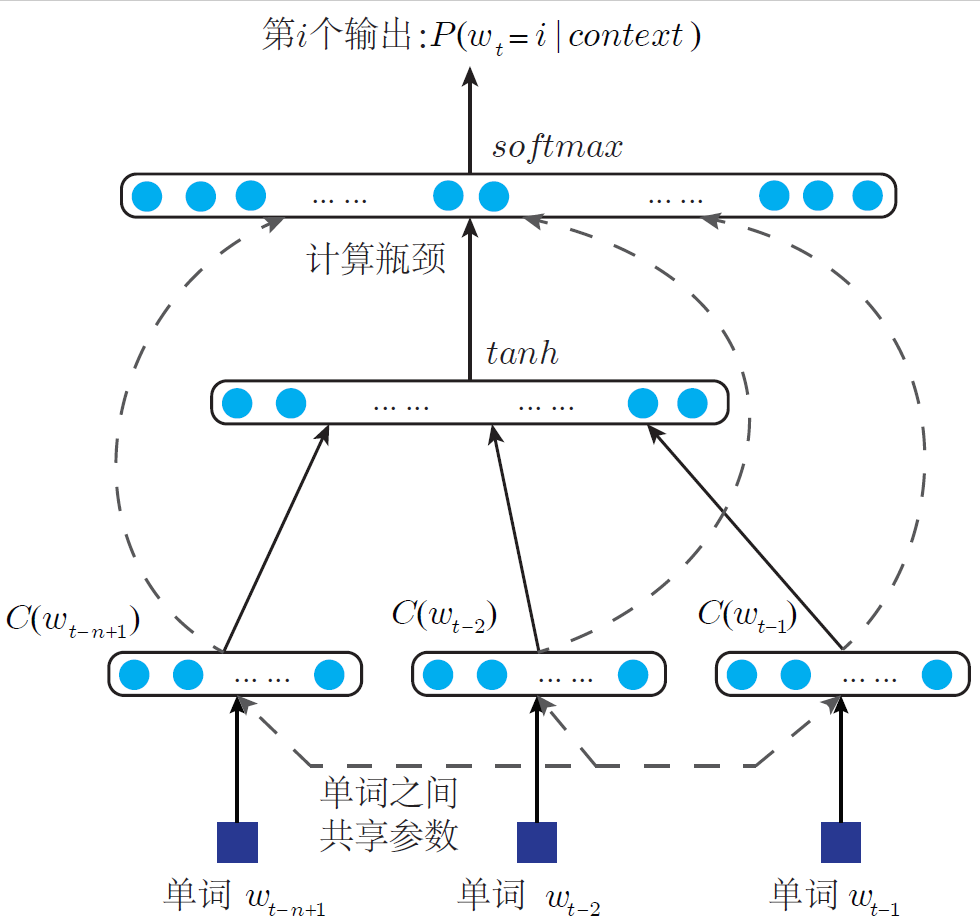
\includegraphics[width=0.68\linewidth]{./figures/nplm2.png}
  \caption{前馈神经网络语言模型。}\label{fig:nplm}
\end{figure}

图.~\ref{fig:nplm} 给出一个典型的 NPLM 语言模型。神经网络语言模型采用普通的三层前馈神经网络结构,其中第一层为输入层。Bengio 提出使用各词的词向量作为输入以解决数据稀疏问题,因此输入层为词$w_{i-(n-1)}, \cdots,w_{i-1} $ 的词向量的顺序拼接:
\begin{equation}\label{equ:we}
  x = [e(w_{i-(n-1)}), \cdots , e(w_{i-2}), e{(w_{i-1})}]
\end{equation}
当输入层完成对上文的表示$x$ 之后,模型将其送入剩下两层神经网络,依次得到隐藏层$h$ 和输出层$y$:
\begin{equation}\label{equ:all_nplm}
\begin{split}
h =& \tanh(Hx+b) \\
y =&Wx + Uh +b'
\end{split}
\end{equation}
其中 $H \in \mathbb{R}^{|h| \times (n-1)|e|}$ 为输入层到隐藏层的权重矩阵,$U \in \mathbb{R}^{|\mathrm{V}|\times (n-1)|h|}$ 为隐藏层到输出层的权重矩阵,$ |\mathrm{V}|$表示词表的大小,$|e|$ 表示词向量的维度,$|g|$ 为隐藏层的维度。$b,b'$ 均为模型中的偏置项。矩阵$W \in \mathbb{R}^{|\mathcal{V}|\times (n-1)|e|}$ 表示从输入层到输出层的直连边权重矩阵。由于$W$ 的存在,该模型可能会从非线性的神经网络退化成为线性分类器。Bengio 等人在文中指出,如果使用该直连边,可以减少一半的迭代次数;但如果没有直连边,可以生成性能更好的语言模型。因此在后续工作中,很少有使用输入层到输出层直连边的工作,下文也直接忽略这一项。如果不考虑$W$ 矩阵,整个模型计算量最大的操作,就是从隐藏层到输出层的矩阵运算$Uh$,后续的模型均有对这一操作的优化。


\subsubsection{循环神经网络}
针对循环神经网络语言模型(Recurrent Neural Network based Language Model,RNNLM)则直接对$P(w_t | w_1,w_2,\cdots,w_{t-1}) $ 进行建模,而不使用公式.~\ref{equ:approx} 对其进行简化~\cite{mikolov2012statistical,DBLP:conf/interspeech/MikolovKBCK10} 。因此,RNNLM 可以利用所有的上文信息,预测下一个词,其模型结构如图.\ref{fig:rnnlm} 所示。
RNNLM 的核心在于其隐藏层的算法:
\begin{equation}
\label{equ:rnn}
h_t =\phi(e(w_t) +Wh_{t -1})
\end{equation}
其中 $\phi$ 为非线性激活函数。但与NPLM 不同,RNNLM 并不采用 n 元近似,而是使用迭代的方式直接对所有上文进行建模。在公式.~\ref{equ:rnn} 中,$h_t$ 表示文本中第 $t$ 个词 $w_t$ 所对应的隐藏层,该隐藏层由当前词的词向量 $e(w_t)$ 以及上一个词对应的隐藏层 $h_{t -1}$ 结合得到。

\begin{figure}
  \centering
  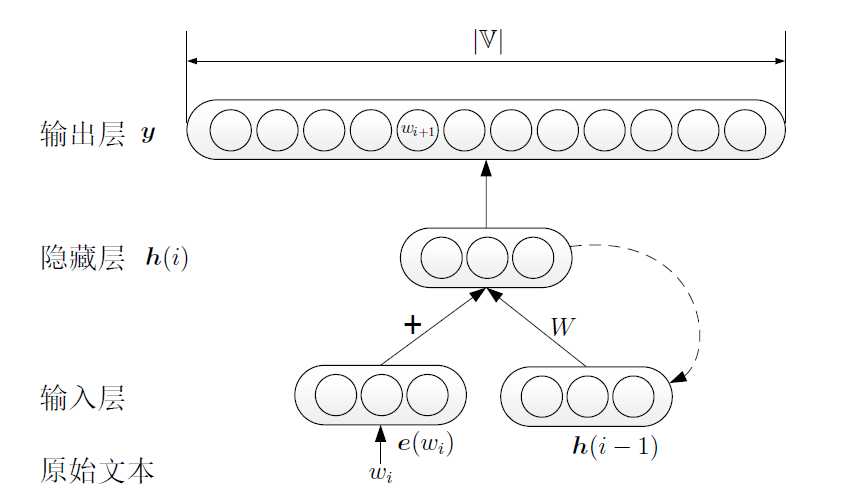
\includegraphics[width=0.68\linewidth]{./figures/rnnlm.png}
  \caption{循环神经网络语言模型(RNNLM)模型结构图}\label{fig:rnnlm}
\end{figure}


隐藏层的初始状态为$h_0$,随着模型逐个读入语料中的词$w_1,w_2,\cdots$, 隐藏层不断地更新为$h_1,h_2,\cdots$ 。根据公式.~\ref{equ:rnn},每一个隐藏层包含了当前词的信息以及上一个隐藏层的信息。通过这种迭代推进的方式,每个隐藏层实际上包含了此前所有上文的信息,相比NPLM 只能采用上文 n 元短语作为近似,RNNLM 包含了更丰富的上文信息,也有潜力达到更好的效果。RNNLM 的输出层计算方法与NPLM 的输出层一致。

\subsubsection{其他网络结构}
除了介绍的两种经典上下建模方法,最近研究提出来可以使用带有门机制(Gate)的RNN来防止模型的长距离依赖问题,例如长短记忆网络(Long Short-Term Memory, LSTM), 门限记忆节点(Gated Recurrent Unit, GRU)和其他网络。

\subsection{完成的工作内容: 大词表问题的优化}
传统的多元分类模型(Softmax):
\begin{equation}
\label{eq:softmax}
\begin{split}
%p(w_i|h)=&\frac{\exp(h^\top v_{w_i})}{\sum_{w_j\in \mathcal{V}}{\exp(h^\top v_{w_j} )}} \\
\log p(w_i|h) &= \theta^w_i h-\log \sum_{w_j\in \mathcal{V}}{\exp(\theta^w_j h)}\\
%\frac{\partial p(w_i|h)}{\partial v_{w_j}}=&p(w_j|h)(\delta_{ij}-p(w_i|h))h^\top\\
\nabla_{\theta^w_j}{\log p(w_i|h)}&= (\delta_{ij}-p(w_i|h))h
\end{split}
\end{equation}
其中 \textit{Kronecker delta} 函数的定义为: $\delta_{ij} = 1$ 如果 $i = j$。 $h$ 是隐藏层输出的向量,并且 $\theta^w$ 是目标端的词向量 $w$~\cite{duda2012pattern}.

其中由于分母是正则项,一旦词表扩大,每次迭代更新都需要计算这一项,是主要的问题所在,所以本课题拟在主要解决该问题所导致的计算费时的问题,在保证计算精度不下降的情况下,提高模型的训练速度。 目前主要的算法分为以下三类: 单词拆分算法、采样估计模型和层次分解模型。


\subsubsection{单词拆分算法}
最直接的算法就是我们放弃使用大词表,转而保留一个较小的词表来保证训练的内存占用和计算效率。那么针对过多的词表外的单词(Out-Of-Vocabulary,OOV),我们可以使用传统的N-gram语言模型来估算其可能的概率分布。这样做一方面保证神经网络模型可以在有限时间内训练完,同时保证模型的最后的测试结果不会很差~\cite{DBLP:journals/csl/Schwenk07}。当我们的词表继续增大的时候,我们会发现训练样本中存在过多的$\langle$unk$\rangle$ 字符,这样使得神经网络的模型训练非常苦难导致效果变得不可接受,所以这种方案只是一定程度上缓解了大词表问题,但是也是一种有效的尝试方案。

\begin{figure}
  \centering
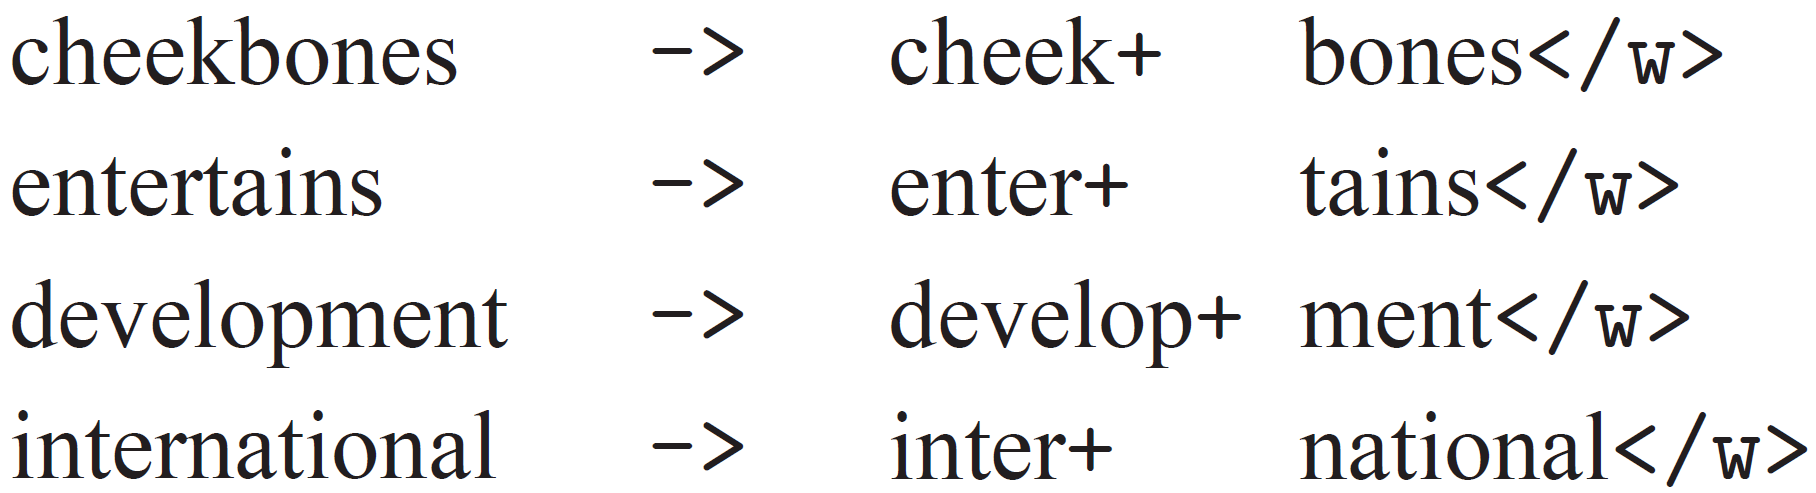
\includegraphics[width=0.6\linewidth]{./figures/subword.png}
\caption{词到子词划分样例.单词背划分成前缀和后缀,其中$+$代表是单词的前缀同时$\langle /w \rangle$是单词的后缀。}\label{fig:subword}
\end{figure}
除了上述方案,目前采用的方案是将单词按照字符级别来划分,可以将一个单词按照字符统计规律划分成任意多个子词。其中二元对编码(byte-pair-encoding,BPE)能将一个单词划分成两部分:前缀(Prefix)和后缀(Suffix)~\cite{DBLP:conf/icassp/Tucker0P94, DBLP:conf/acl/SennrichHB16a,Gage:1994:NAD:177910.177914},如图.~\ref{fig:subword} 所示。由于划分规则是从训练数据中学习到的,我们可以指定需要缩减的词表大小,该算法的动态适应性很强,目前主流的机器翻译模型都采用这个方案~\cite{DBLP:journals/corr/JozefowiczVSSW16}。尽管如此,我们仍然需要看到它这样的解构操作依然带来了一定的损失,因为句子的长度增倍了,对RNN的长距离关系学习能力提出了更高的挑战~\cite{DBLP:conf/aaai/KimJSR16}。

\subsubsection{采样估计模型}
目前采用的采样算法主要是针对概率规约那一项进行概率估计,其中著名的算法有:重要性采样(Importance Sampling)~\cite{DBLP:journals/tnn/BengioS08},噪声差分估计(Noise Contrastive Estimation, NCE)~\cite{DBLP:conf/icml/MnihT12}和Blackout 采样算法~\cite{DBLP:journals/iclr/JiVSAD15}。第一种算法在实验中被证明模型无法收敛,目前主要使用的后面两种算法。

对于噪声差分估计算法来说,模型需要学习将正确的单词 $w_0$ 与随机生成的单词 $\{w_1\cdots w_k\}$做一个二元分类。 其中 $w_0$ 训练样本中真正的下一个单词, $\{w_1\cdots w_k\}$ 是采用先验分布  $q(w)$产生的随机噪声单词. 正例归一化后的概率和所有负例联合概率的公式可以写成:
\begin{equation}\label{equ:nce}
\begin{split}
  \tilde{p}(y=1|h)=&\frac{\exp( \theta^w_0 h)}{ \exp( \theta^w_0 h)+k *q(w_0)}\\
  \tilde{p}(y=0|h)=&\prod_{i=1}^{k}\frac{k *q(w_i)}{\exp( \theta^w_i h)+k *q(w_i)}\\
\end{split}
\end{equation}
需要注意的是 $\tilde{p}(y=0|h)$ 需要对 $k$ 个噪声样本做加法运算而不是对整个词表单词进行的。 这样的话该算法的计算机复杂度就是$\mathcal{O}(k)$,和整个词表的大小无关了。除此之外,最近提出的Blackout采样算法针对噪声概率归一化的时候与当前上下文的相关,对NCE算法进行了进一步修改~\cite{DBLP:journals/iclr/JiVSAD15}。

\subsubsection{层次分解模型}
目前主要的策略分为: 基于类别的多元分类模型(class-based hierarchical softmax, cHSM)和基于二叉树的二元分类模型(class-based hierarchical softmax, tHSM)。图.~\ref{fig:case_hsm}展示了第一种算法的示例,图.~\ref{fig:tree_hsm}展示了第二种算法的示例。
\begin{figure}
  \centering
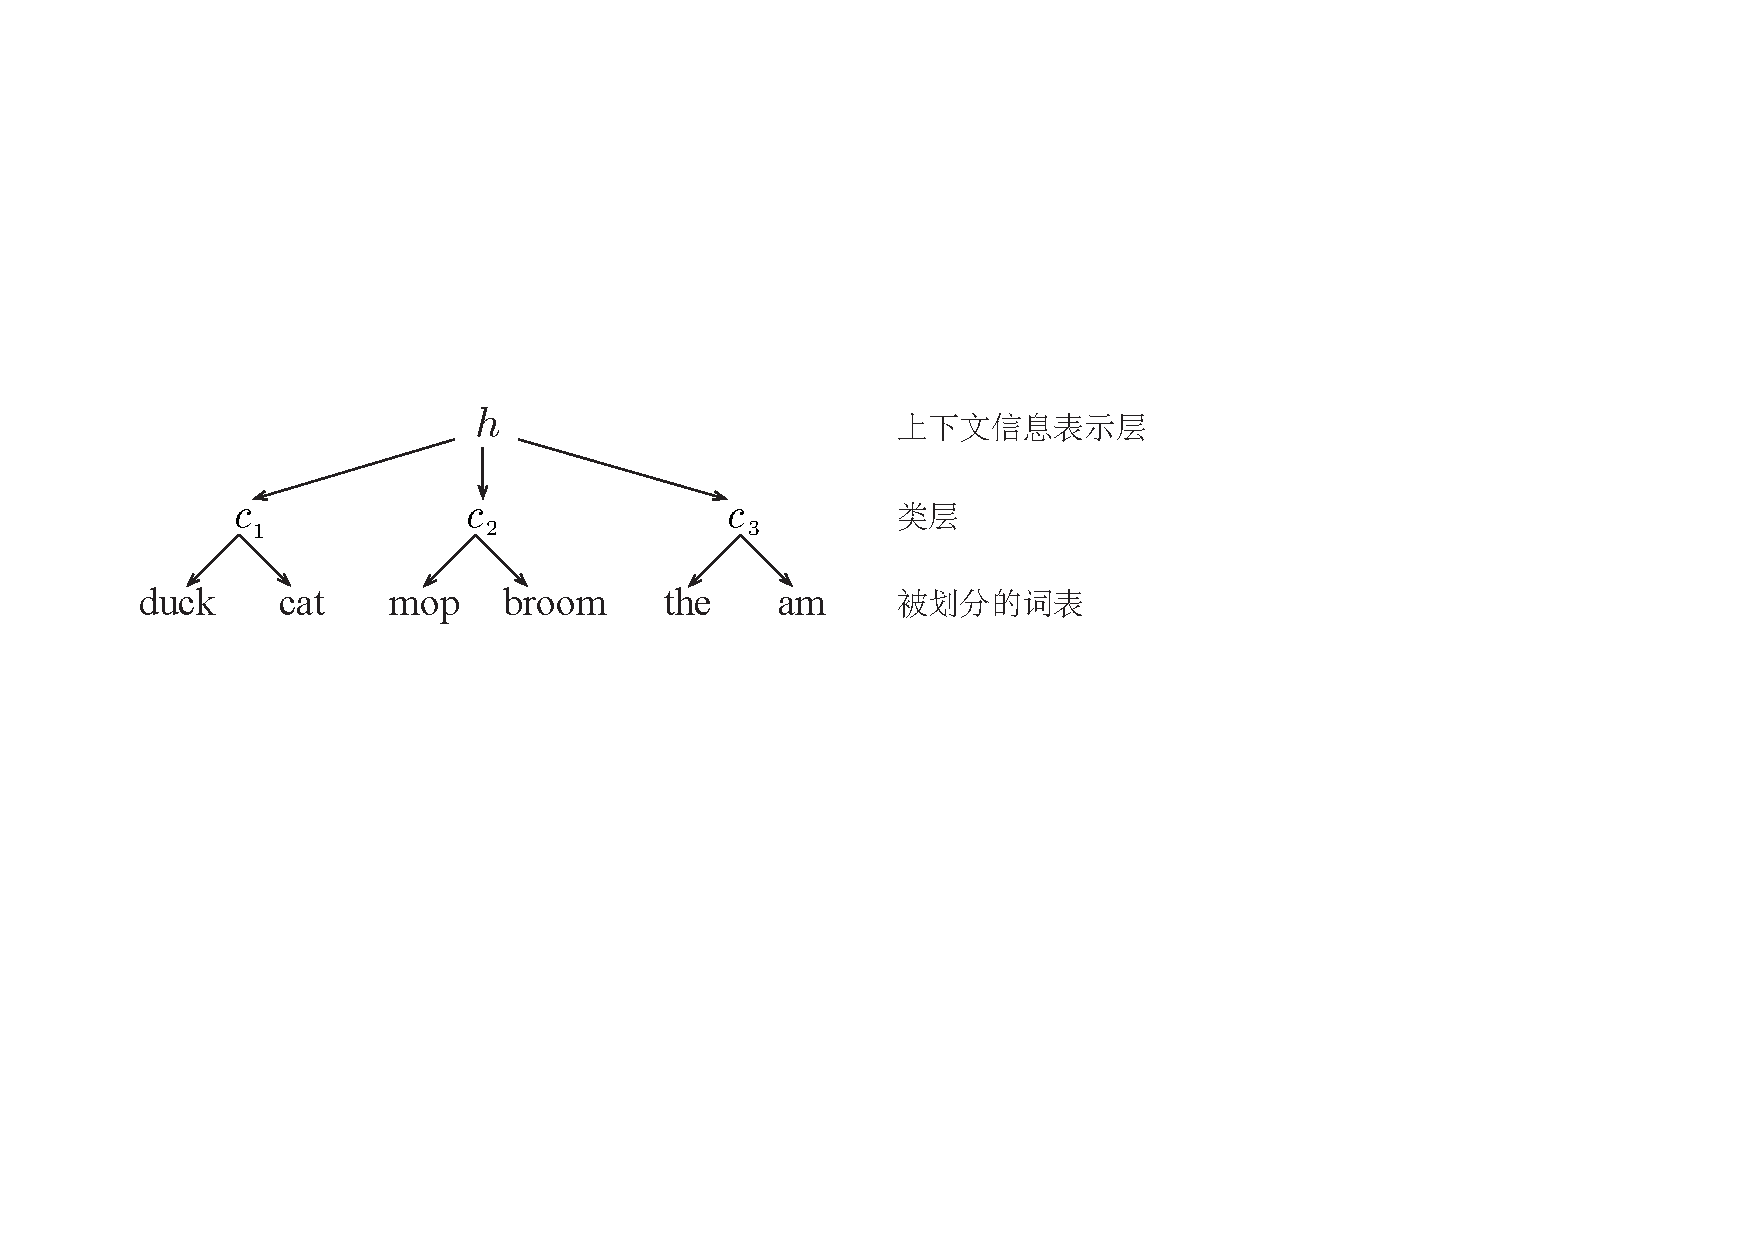
\includegraphics[width=0.65\linewidth]{./figures/case_chsm.pdf}
\caption{cHSM算法可视化模型。其中词表 \{duck,cat,mop,broom\} 被划分成:\{duck,cat\},\{mop,broom\}.}\label{fig:case_hsm}
\end{figure}



\begin{figure}
  \centering
    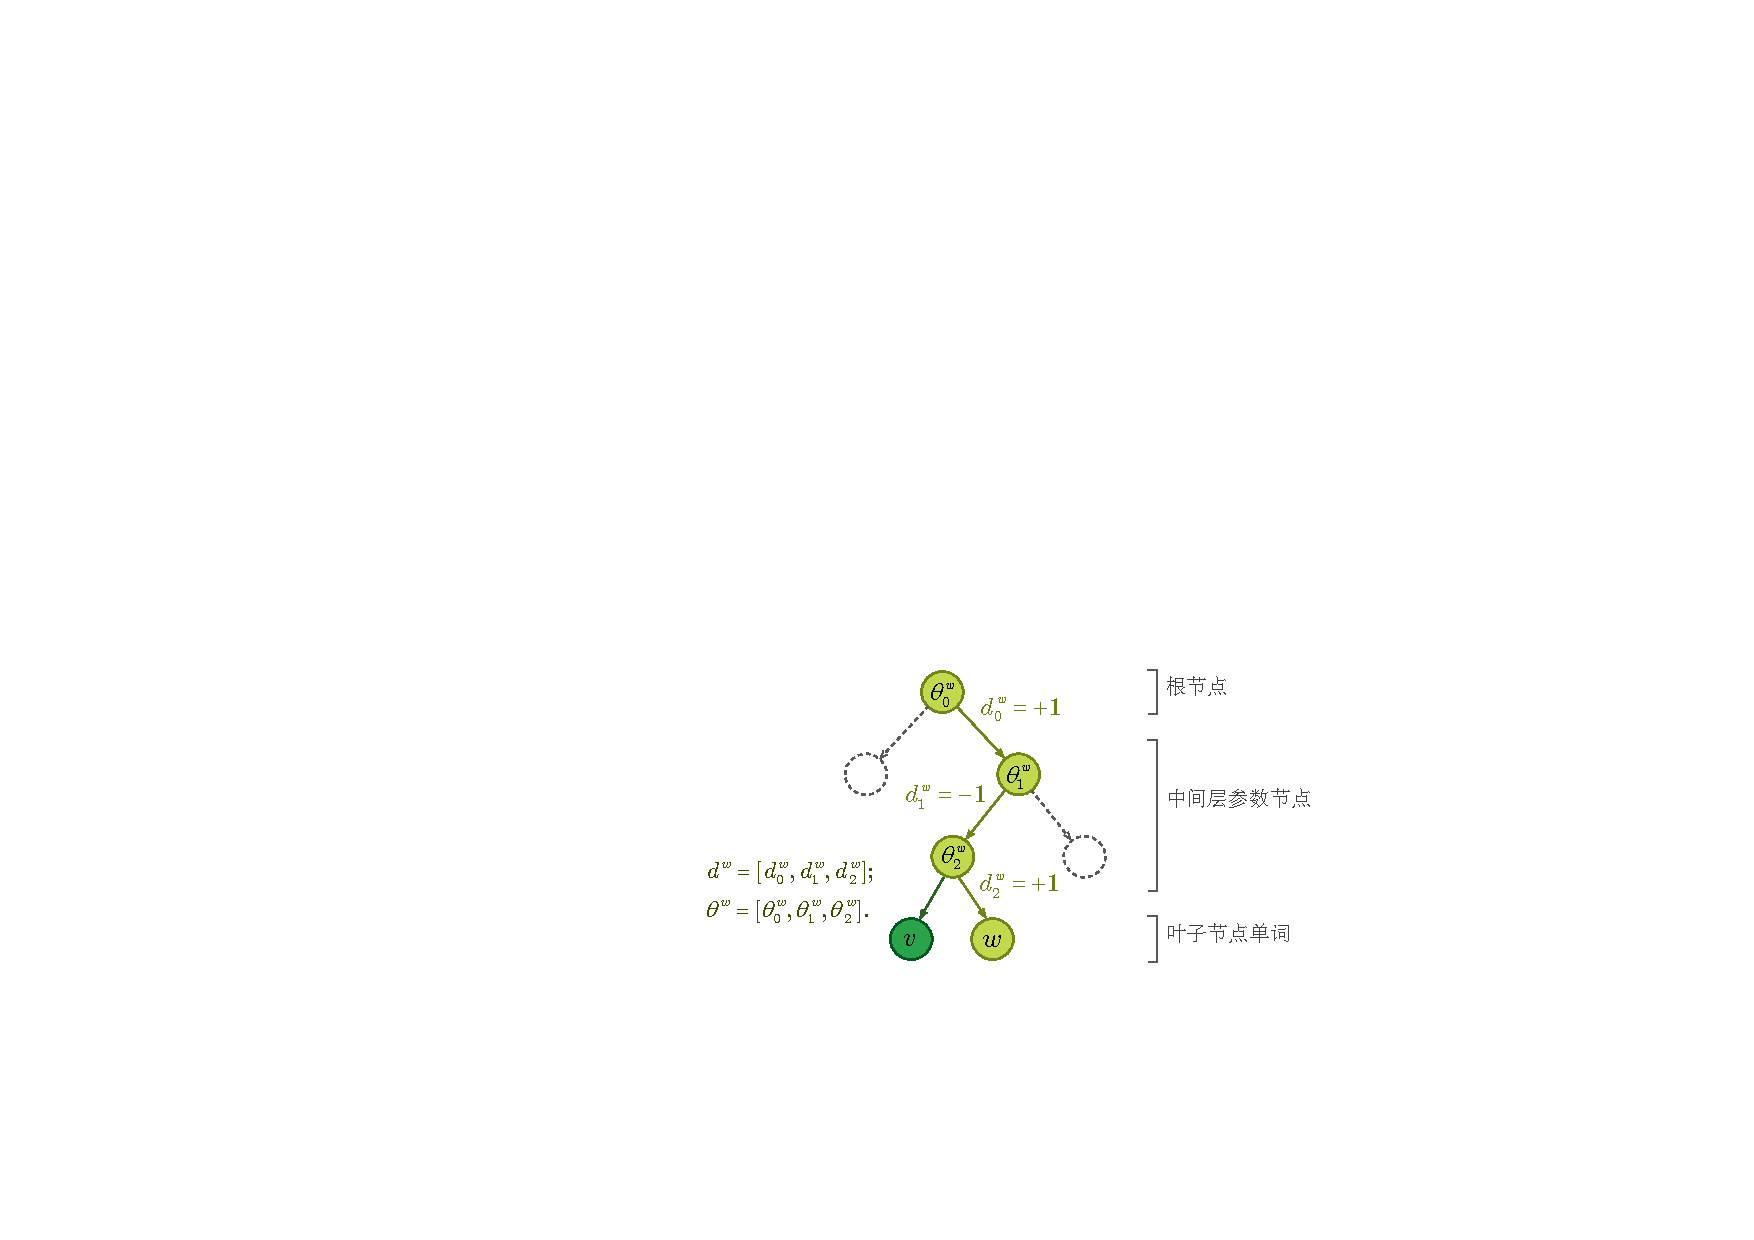
\includegraphics[width=0.7\linewidth]{./figures/thsm.pdf}
\caption{树状层次概率模型. 内部参数 $\theta_i^w$, 边 $d_i^w$ 并且单词在树的叶子节点上. 除此之外, 加粗的那条路径从根节点到叶子节点 $w$ 被定义为参数对 $(d^w,\theta^w)$。其中 $d^w$ 是一个向量, $\theta^w$ 是一个参数矩阵. 例如, $d^w=[-1,+1,-1]$ , $d^{v}=[-1,+1,+1]$.}\label{fig:tree_hsm} %
\end{figure}

 \begin{equation}
p(d^w_i|\theta_{i}^w,h) =\sigma(\theta_{i}^w h)^{d_i^w}\times[1-\sigma(\theta_{i}^w h)]^{1-{d_i^w}},d_i^w \in [0,1]
\end{equation}
 \begin{equation}
p(d^w_i|\theta_{i}^w,h) =\sigma(\theta_{i}^w h)^{d_i^w}, d_i^w \in [-1,1]
\end{equation}
\begin{equation}
p(d^w_i=\pm 1|\theta_{i}^w,h) = \sigma({d_i^w}\theta_{i}^w h)
\end{equation}

一个单词的概率 $w$:
\begin{equation}\label{equ:pw}
\begin{split}
 \log p(w|h)=&\log\prod_{i=0}^{l^w-1} p(d^w_i|\theta_{i}^w,h) = \sum_{i=0}^{l^w -1} \log\sigma(d_i^w \theta_{i}^w h)\\
 =&\log\sigma({d^w}^\top \theta^w h)=\zeta(- {d^w}^\top \theta^w h )
 \end{split}
\end{equation}
$\zeta(z)$ 表示 softplus 函数: $\zeta(z)= \log (1+\exp(z))$.
树状模型的优点:
\begin{equation}
\sum_{w\in \mathcal{V}}{p(w|h)}=\sum_{w \in \mathcal{V}}\sum_{i=0}^{l^w-1}{\sigma(d_i^w\theta_{i}^w h)}=1.
\end{equation}


\begin{figure}
  \centering
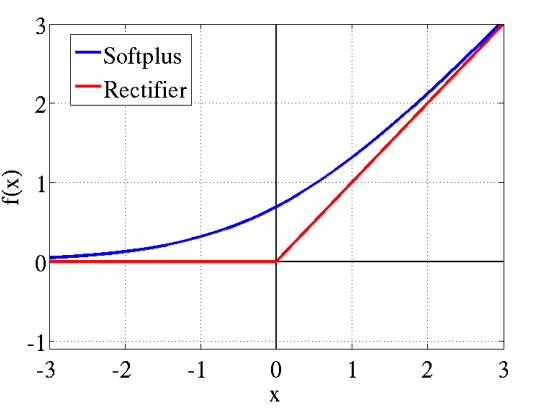
\includegraphics[width=0.5\linewidth]{./figures/softplus.png}
\caption{Softplus和ReLU函数的示意图。}\label{fig:soft}
\end{figure}

\section{关键技术或难点}

\subsection{关键技术或难点:复杂上下文建模方案}
依照上章节的分析,本章节主要介绍我们实验中所要涉及的模型,主要是各种循环神经网络的变种 \cite{DBLP:conf/icml/JozefowiczZS15}: 普通循环神经网络节点、长短记忆网络(Long shrot-term memory, LSTM)~\cite{DBLP:journals/taslp/SundermeyerNS15} 和门限记忆节点(Gated Recurrent Unit, GRU) \cite{DBLP:conf/nips/ChungKDGCB15}。 LSTM的计算公式定于如下 \cite{DBLP:journals/neco/HochreiterS97}:
\begin{itemize}
\item 输入门: 控制当前输入 $x_t$ 和前一步输出 $h_{t−1}$ 进入新的 cell 的信息量:$i_t=\sigma(W^i x_t+U^i h_{t-1}+b^i)$
\item  忘记门:决定是否清楚或者保持单一部分的状态$f_t=\sigma(W^f x_t+U^f h_{t-1}+b^f)$
\item  变换输出和前一状态到最新状态$g_t=\phi(W^g x_t+U^g h_{t-1}+b^g)$
\item  输出门: 计算 cell 的输出$o_t=\sigma(W^o x_t+U^o h^{t-1}+b^o)$
\item  cell 状态更新步骤:计算下一个时间戳的状态使用经过门处理的前一状态和输入:$s_t=g_t\odot i_t+s_{t-1}\odot f_t$
\item  最终 LSTM 的输出:使用一个对当前状态的 tanh 变换进行重变换:$h_t=s_t\odot \phi(o_t)$
\end{itemize}
其中$\odot$ 代表对应元素相乘(Element-wise Matrix Multiplication), 函数 $\phi(x), \sigma(x)$ 的定义如下:
\begin{equation}\label{equ:tanh}
  \phi(x)=\frac{e^x-e^{-x}}{e^x+e^{-x}},\sigma(x)=\frac{1}{1+e^{-x}}
\end{equation}

\begin{figure}
  \centering
  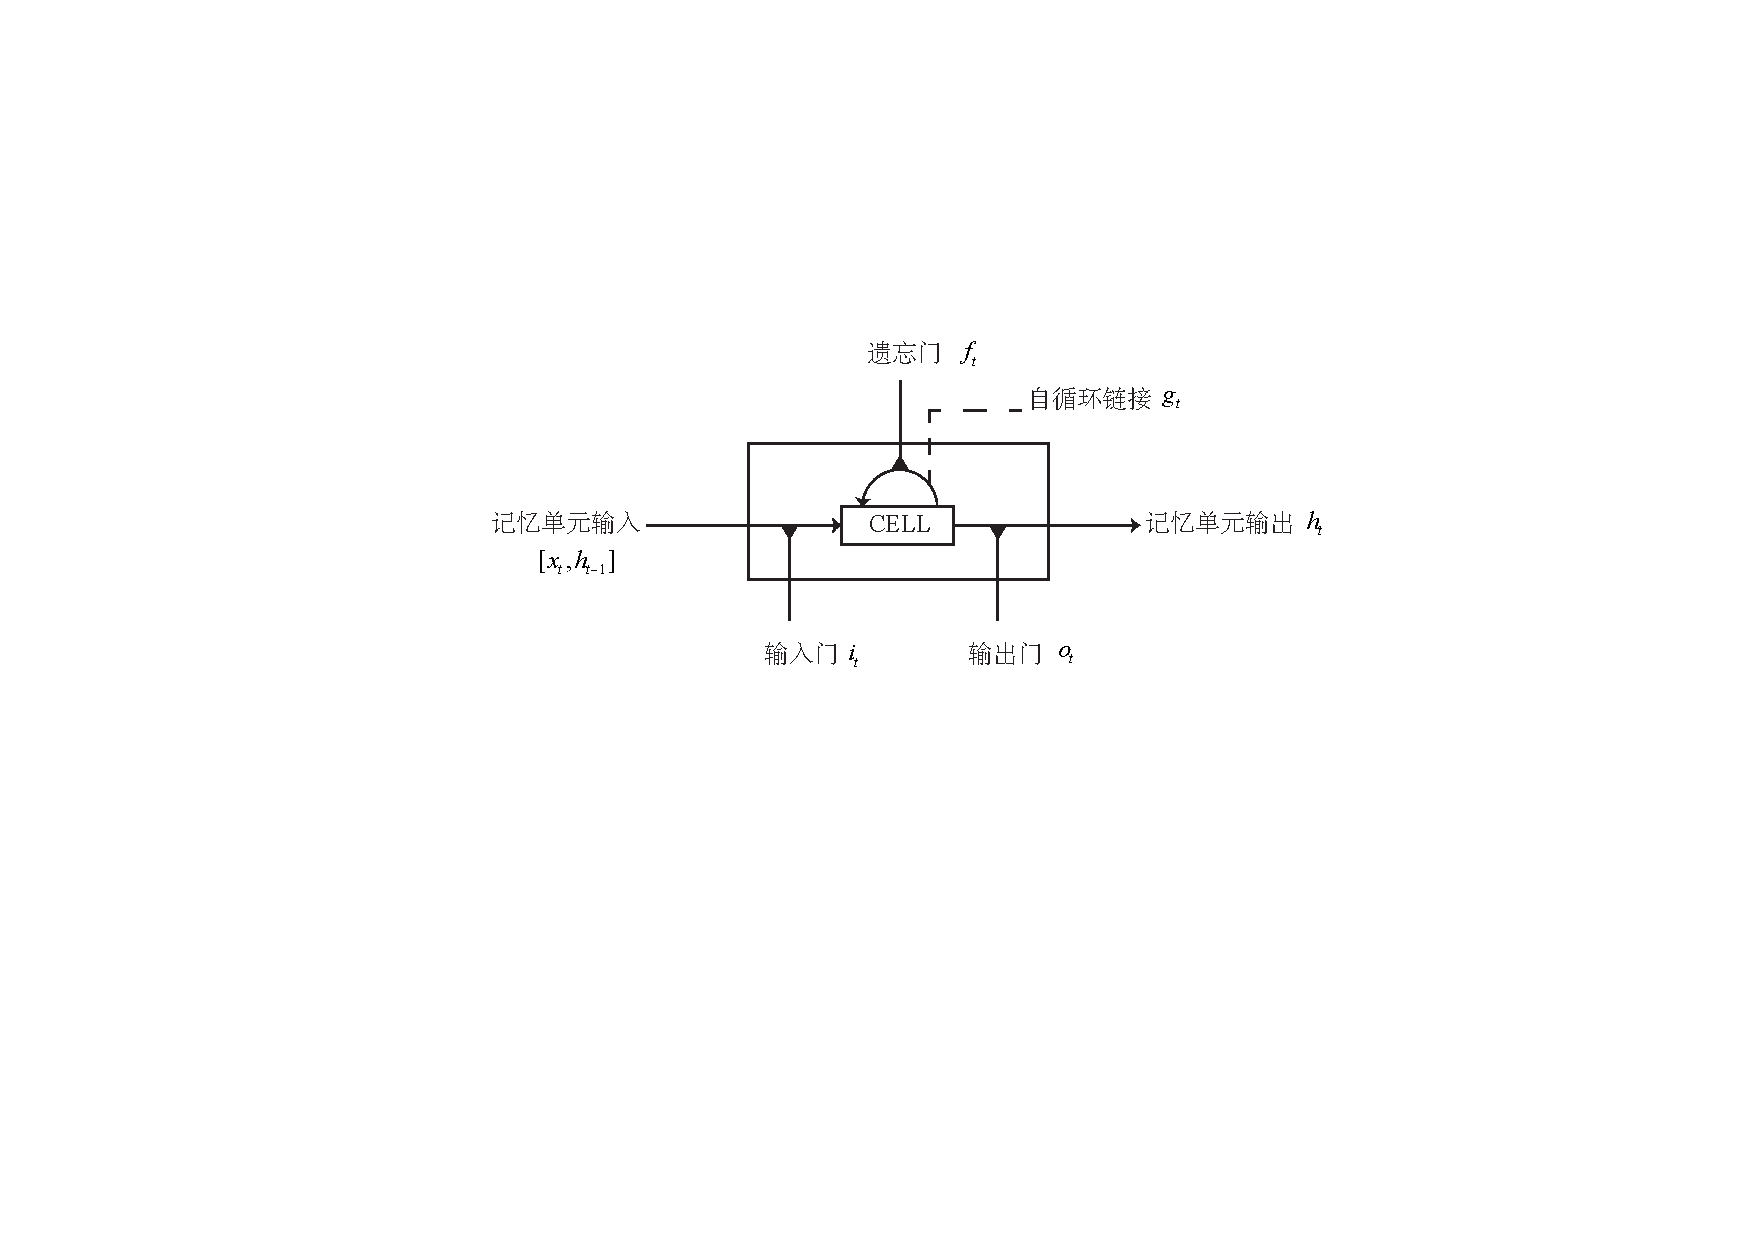
\includegraphics[width=0.7\linewidth]{./figures/lstm.pdf}
  \caption{LSTM 模型}\label{fig:lstm}
\end{figure}


GRU 可以看成是 LSTM 的变种,GRU 把 LSTM中的 遗忘门和输入门用更新门来替代。 把 cell state 和隐状态 $h_t$ 进行合并,在计算当前时刻新信息的方法和 LSTM 有所不同。 下图是GRU更新 $h_t$ 的过程\cite{DBLP:journals/corr/Pezeshki15}, 具体定义如下:
\begin{itemize}
\item 更新门 $z_t$: 定义保存多少以前的信息:$z_t = \sigma ( W^z x_t+ U^z h_{t-1}  )$

\item 重置门 $r_t$: 决定保留多少输入信息:$r_t = \sigma(W^r x_t  + U^r h_{t-1}  )$

\item 节点内部更新值$\tilde h_t $: 其次是计算候选隐藏层(candidate hidden layer) $\tilde h_t$,这个候选隐藏层 和LSTM中的$\tilde c_t$是类似,可以看成是当前时刻的新信息,其中$r_t$用来控制需要 保留多少之前的记忆,如果$r_t$为0,那么$\tilde h_t$只包含当前词的信息:$\tilde h_t  = \tanh (W^h x_t  + U^h(h_{t-1} \odot r_t) )$

\item 隐藏层输出值$h_t$: 最后$z_t$控制需要从前一时刻的隐藏层 $h_{t-1}$ 中遗忘多少信息,需要加入多少当前 时刻的隐藏层信息$\tilde h_t$,最后得到$h_t$,直接得到最后输出的隐藏层信息, 这里与LSTM的区别是GRU中没有 输出门:$h_t = (1-z_t)\odot \tilde h_t  + z_t \odot h_{t-1}$
\end{itemize}
如果重置门接近0,那么之前的隐藏层信息就会丢弃,允许模型丢弃一些和未来无关 的信息;更新门 控制当前时刻的隐藏层输出$h_t$需要保留多少之前的隐藏层信息, 若$z_t$接近1相当于我们之前把之前的隐藏层信息拷贝到当前时刻,可以学习长距离依赖。 一般来说那些具有短距离依赖的单元重置门比较活跃(如果$r_t$为1,而$z_t$为$0$ 那么相当于变成了一个标准的RNN,能处理短距离依赖),具有长距离依赖的单元更新门比较活跃。

\begin{figure}
  \centering
  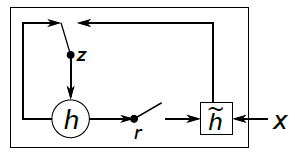
\includegraphics[width=0.5\linewidth]{./figures/gru.png}
  \caption{GRU模型示意图}\label{fig:gru}
\end{figure}


\subsection{关键技术或难点:层次概率模型}
大词表问题,主要是对softmax如何建模的问题。在本课题中,我们探讨 cHSM 和 tHSM 两种不同的方案所带来的影响和优劣。

假设语料中的每一个词样本属于且只属于一个类,在此基础上计算词样本在语料中的分布时,可以先计算类的概率分布,然后在所属类上计算当前词的概率分布,于是可将公式.~\ref{eq:softmax} 转化为:
  \begin{equation}
  \begin{split}
p(w|h)=&p^c(\mathcal{C}(w)|h)\cdot p^w(w|\mathcal{C}(w),h) , w\in \mathcal{C}(w),\\
&\mathcal{V}=\bigcup _{i = 1}^\mathcal{C}{c_i},\quad  c_i \bigcap c_j=\phi, \text{If}\quad i\ne j, \\
\end{split}
\end{equation}
此时,训练一个词样本的计算复杂度正比于: $O =HC$。 式中,$C$ 为语料中所有词的分类数,可根据语料中词的词频进行划分。 当$C$ 取$1$ 或取词典大小$V$ 时,此结构等同于标准的RNN 结构。 由于$C \ll V$,该结构训练的softmax 降低了计算复杂度。

\begin{table}
  \centering
  \caption{cHSM 方法在Wikitext-2 数据集性能评测.\label{table:clustering}}
  \begin{tabular}{lccccc} \toprule
  &Branch& Epoches& PPL \& WER &Time(ms)\\\midrule
  &10/3330&193&211.51 / 77.41 &788\\
  &20/1664&252&220.01 / 77.71&549\\
  &40/832&273&236.56 / 77.95&302\\
  &80/417&291& 241.12 / 78.25&170\\
  &160/208&301&247.25 / 79.21&93\\
  &182/183&339&253.35 / 79.92&86\\
\bottomrule
\end{tabular}
\end{table}


Mikolov曾提出使用基于二叉树的层级softmax模型来加速的训练方案,加速比能达到理论的最大速度,但是当时提出的背景是基于CPU构建的,如今越来越多的算法随着应用领域的推广,需要在并行度更高的GPU上进行计算,因此基于GPU进行建模的tHSM尚未被研究提及,需要在本文中研讨。
\section{下一阶段工作计划}
当我们使用多层分类模型的时候,我们就需要将单词按照模型的架构进行划分。其中对于cHSM模型,我们有以下策略可以使用:1) 基于词频划分类别; 2) 基于Bigram 的布朗聚类(Brown clustering) 进行划分;3)按照word-embedding 的词向量信息进行聚类。另外,我们还需要注意的是,各个类别可以包含不同的数量的单词,也可以包含数量相同的单词。对于后者,我们考虑的划分模型就是基于交换算法(Exchange Algorithm), 以此来保证获得近似的最优解。

\subsection{存在的问题}
目前存在的问题主要是两点:模型仍然计算很复杂需要使用更底层语言来加速计算,和目前采用的聚类算法比较费时间。

由于我们选择的建模平台是python平台,好处是可以使用许多现成的已有的框架。并且python语法简单,矩阵计算库numpy和scipy更成熟,便于调试。另一方面,我们采用的建模语言是theano框架,它的底层计算都是调用BLAS计算库,或者直接调用基于GPU的CUDA的CuBLAS计算库。虽然这样做便于在前期模型建立阶段能方便尝试各种设计方案,但是他的计算瓶颈在python解释器对代码的缓慢执行,所以如果能将部分模型组件使用CUDA语言重写。那样的话,我们的模型能接受一定的组合排列的可能性,同时计算速度能得到极大提升。这也是许多目前流行框架发展的方向,有些框架更超前。例如MXNET直接使用C++语言建立深度模型,他的计算效率也是目前已知的框架中最快的。因此,考虑到目前的thenao计算瓶颈,我们想将RNN的框架使用CUDA语言重构,基于CuDNN库开发的样板,帮助我们在他基础上改进。

另一方面,目前采用的聚类算法计算非常费时,尤其是当我们希望进行多层次聚类的时候,我们需要花费数周时间来获得结果。这样的缓慢的计算效果是无法接受的,经过针对代码的调试,我们发现计算瓶颈在算法初始化的时候,计算两两单词之间的距离,它花费了90\%的计算时间。如果能存在有效的初始化算法,而不是挑选尽可能高精度的聚类模型,那么实验进度和试验结果就可以针对多组参数调试。
\subsection{尚未完成的工作}
\begin{enumerate}
\item 大规模实验数据分析验证算法;
\item 优化模型速度,用底层语言封装模型,以达到最好的效果;
\item 实验和评价不同聚类算法的效果;
\item 讨论和研究不同语言模型优化方案的优缺点,以及使用场景。
\end{enumerate}
\subsection{解决问题的技术思路或措施}
\begin{enumerate}
\item 大规模实验数据分析验证算法:目前已经找到三个标准文本数据集,需要重写数据处理算法,这样保证模型能正常运算和收敛;
\item 优化模型速度,用底层语言封装模型,以达到最好的效果:学习CUDA语言,并着手构建基于深度学习的模型框架;
\item 实验和评价不同聚类算法的效果:调研可用的层次聚类算法并进行测试和实验检验;
\item 讨论和研究不同语言模型优化方案的优缺点,以及使用场景:提出不同的实验评价指标,观察不同模型的结果,并分析其背后的原因。
\end{enumerate}
% 参考文献
\cleardoublepage
\phantomsection
\addcontentsline{toc}{chapter}{参考文献}
\nocite{*}
\bibliography{data/bibs}
\cleardoublepage

% 附录
\appendix
% !Mode:: "TeX:UTF-8"
\chapter{常见问题}
\label{chapter-faq}
\begin{enumerate}
\item 本模板如何使用?
\label{faq-howtouse}
\begin{itemize}
    \item 按照第2章的要求,先下载和安装相应的软件,推荐使用\TeX{}Live2012或更新的版本;
    \item 下载cls文件;
    \item 使用tex的编辑器或其他编辑器,编写论文,注意保存为UTF-8编码;
    \item xelatex编译。
\end{itemize}
注意:\TeX{}Live2012的ISO镜像在\href{http://buaabt.cn/showtopic-214948.aspx}{未来花园BT站}上
有相应的种子可下载,亦可从TUG的\href{http://www.tug.org/texlive/acquire-iso.html}{官方网站}上下载。
\item Windows下的msmake.bat如何使用?
\label{faq-msmake}
\begin{itemize}
    \item 使用Windows的CMD命令行,进入到msmake.bat所在目录;
    \item 键入~msmake~后会显示相应的帮助文件;
    \item 按照所显示的相关信息再键入相应命令即可。
\end{itemize}
注意:由于此批处理文件为编者自行编写,学识有限,代码有许多不如人意之处,
如对此批处理文件有问题可直接邮件联系我(mrpeng000@gmail.com)即可。
\item 使用TexLive如何更新?
\label{faq-texliveupdate}
TUG官方推荐\TeX{}Live通过镜像站进行更新,具体步骤为:
\begin{itemize}
    \item 在“开始”目录下的TeXLive2012文件夹下,找到有TeX Live Manage程序;
    \item 在菜单“tlmgr”下选择“载入其他仓库”,选择最近的仓库即可(如果是北航校内用户并能够
    访问到\href{http://mirror.buaa.edu.cn/}{北航开源镜像站}的话,可以在仓库地址中
    输入\texttt{http://mirror.buaa.edu.cn/CTAN/systems/texlive/tlnet/});
    \item 按照目录选择更新。
\end{itemize}
\end{enumerate}

% !Mode:: "TeX:UTF-8"
\chapter{联系我们}


% 附页标题样式
\backmatter

% 附页
% !Mode:: "TeX:UTF-8"
\chapter{攻读博士/硕士学位期间取得的学术成果}
% 此处标题及内容请自行更改
\noindent 发表论文:
\begin{enumerate}

\item
Gang Bai and Yue Qi. An Interactive 3D Exhibition System with
 Global Illumination for Digital Museum. In Lecture Notes in
 Computer Science, 2009, Volume 5670, Learning by Playing.
Game-based Education System Design and Development, Pages 85-92.

\item
Hu Yong, Qi Yue and Bai Gang. Modeling and Editing Isotropic BRDF.
In proceedings of the Second International Conference on Modeling,
Simulation and Visualization Methods (WMSVM). 15-16 May, 2010,
Sanya, China. Pages 74-77.

\end{enumerate}


% !Mode:: "TeX:UTF-8"
\chapter{致谢}

% !Mode:: "TeX:UTF-8"
\chapter{作者简介}
  xxxx 年 xx 月 xx 日出生于 xx 省 xx 县。

  xxxx 年 9 月考入 xx 大学 xx 系 xx 专业,xxxx 年 7 月本科毕业并获得 xx 学士学位。

  xxxx 年 9 月免试进入 xx 大学 xx 系攻读 xx 学位至今。
\end{document}
